\subsection{Directional diffusion}

The regular diffusion approach will present noticeable artifacts. These typically occur at high-contrast edges of the image. Because the diffusion kernel equally weighs pixels from all directions it creates a blur effect and is unable to properly propogate edges into the unknown regions. This effect can be seen in figure \ref{fig:artifacts}. To help resolve this problem we would like to use motion kernels that weigh pixels from certain directions more heavily. To do this we divide the image into separate patches. For each patch we infer the general directionality by using a heuristic. We take a motion-kernel and rotate it according to the directionality found. Then we apply this kernel to do the inpainting for that specific patch. By doing so, we are able to resolve some of the artifacts that are generated by regular diffusion.

\subsubsection{test}

\begin{figure*}[h]
	\centering
	\begin{subfigure}[b]{0.49\textwidth}
		\centering
		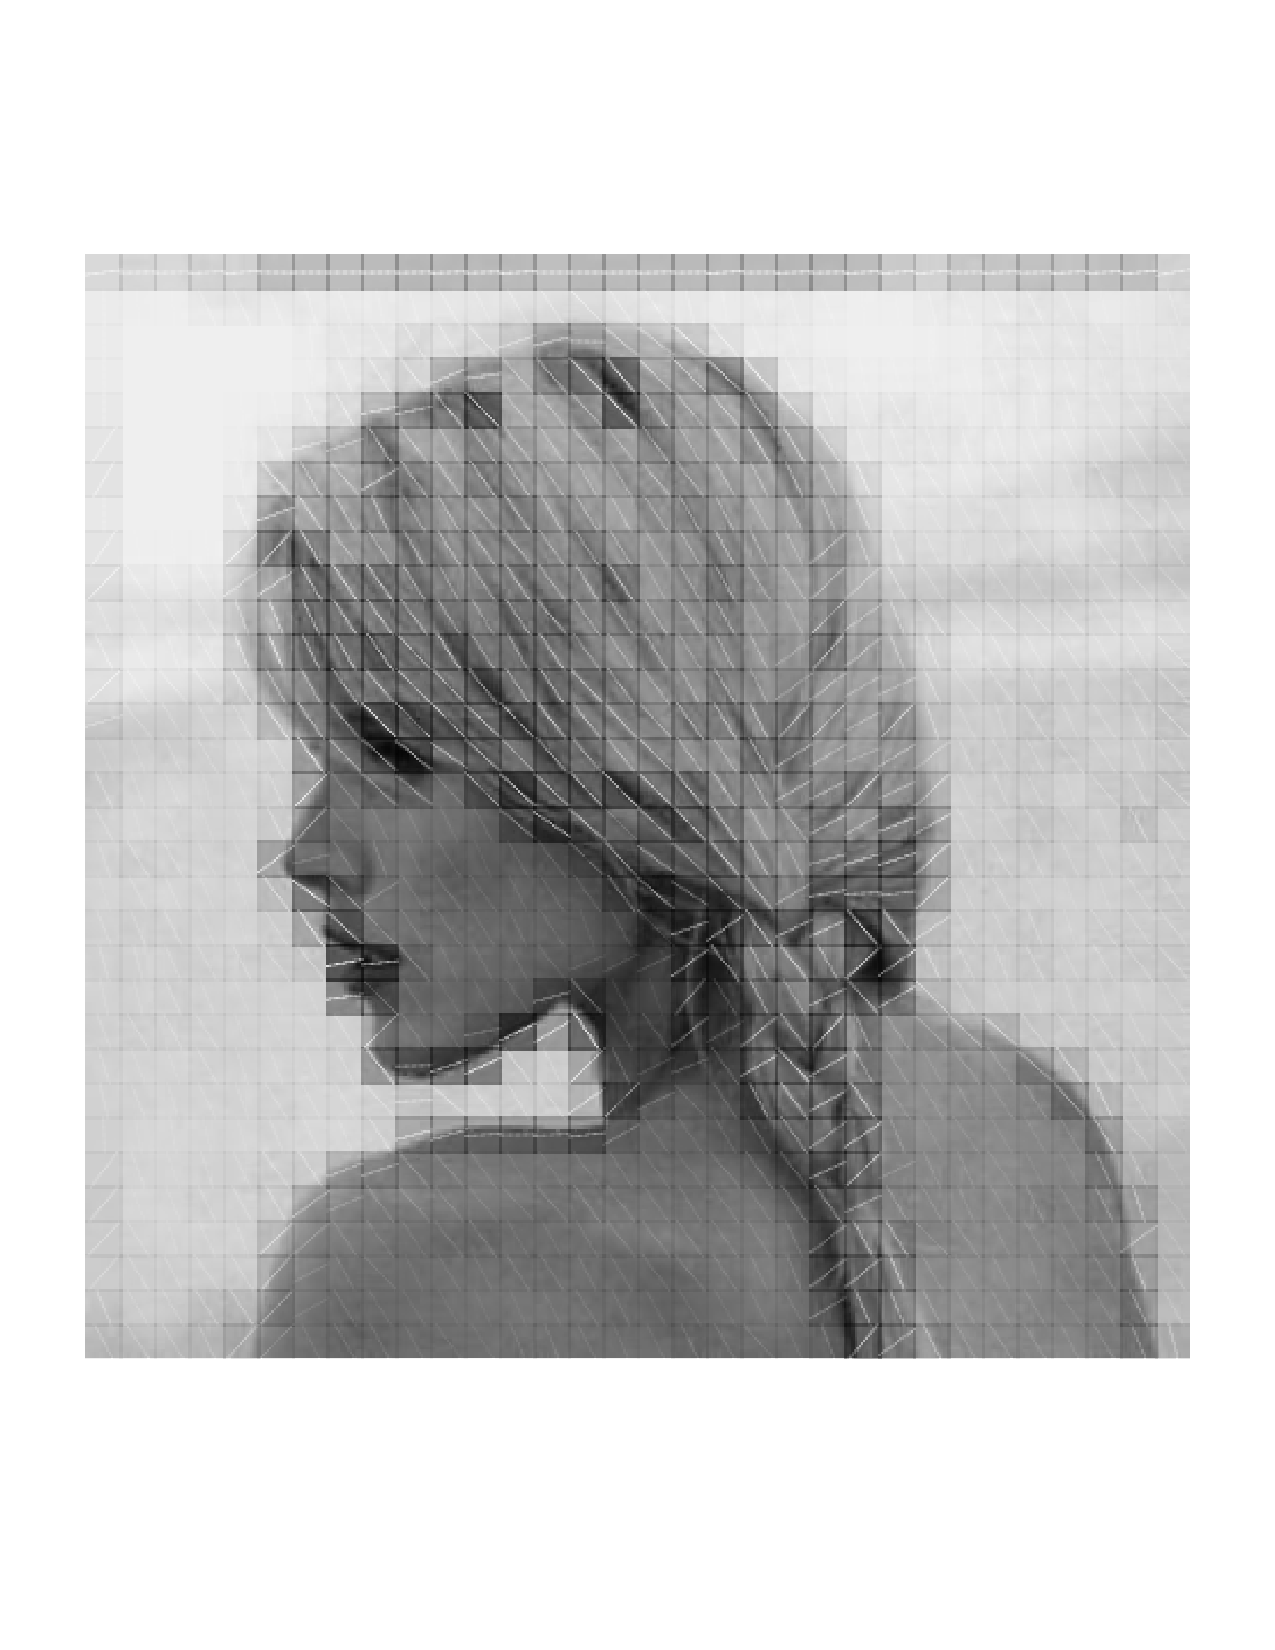
\includegraphics[width=0.9\textwidth]{figures/directional_claudia}
		\caption{The claudia image.}
		\label{fig:claudia}
	\end{subfigure}
	\begin{subfigure}[b]{0.49\textwidth}
		\centering
		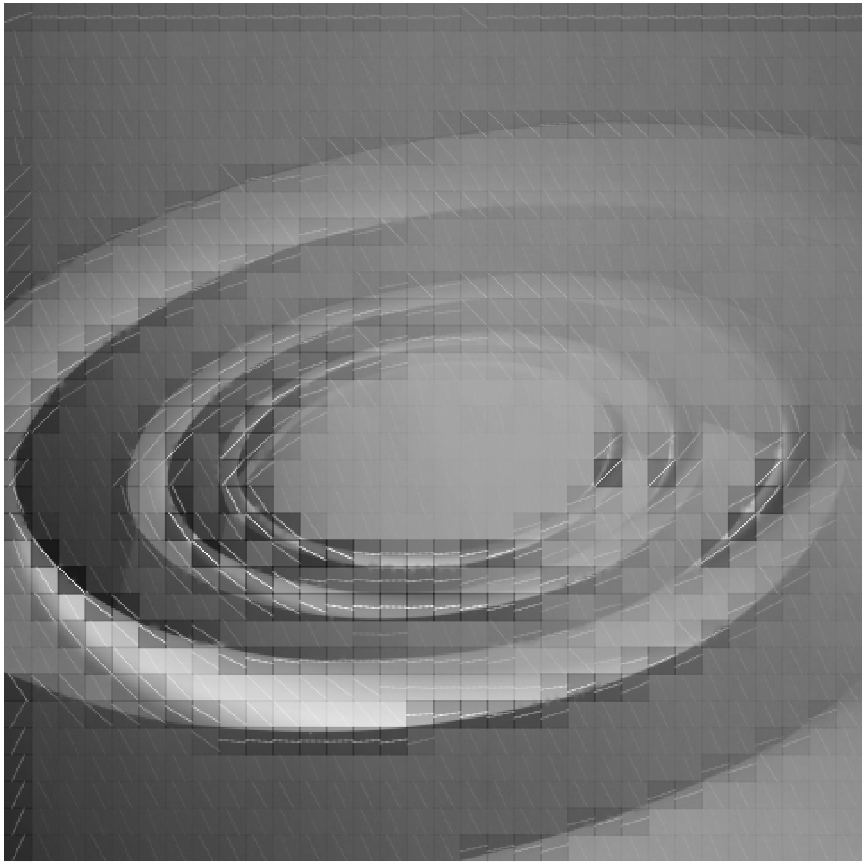
\includegraphics[width=0.9\textwidth]{figures/directional_spiral}
		\caption{The spiral image.}
		\label{fig:spiral}
	\end{subfigure}
	
	\caption{The directionality of 16x16 patches shown as white lines after the first diffusion stage.}
	\label{fig:directionality}
\end{figure*}